\section{Introduction}




\begin{figure}[t]
    \centering
    % \vspace{-20pt}
    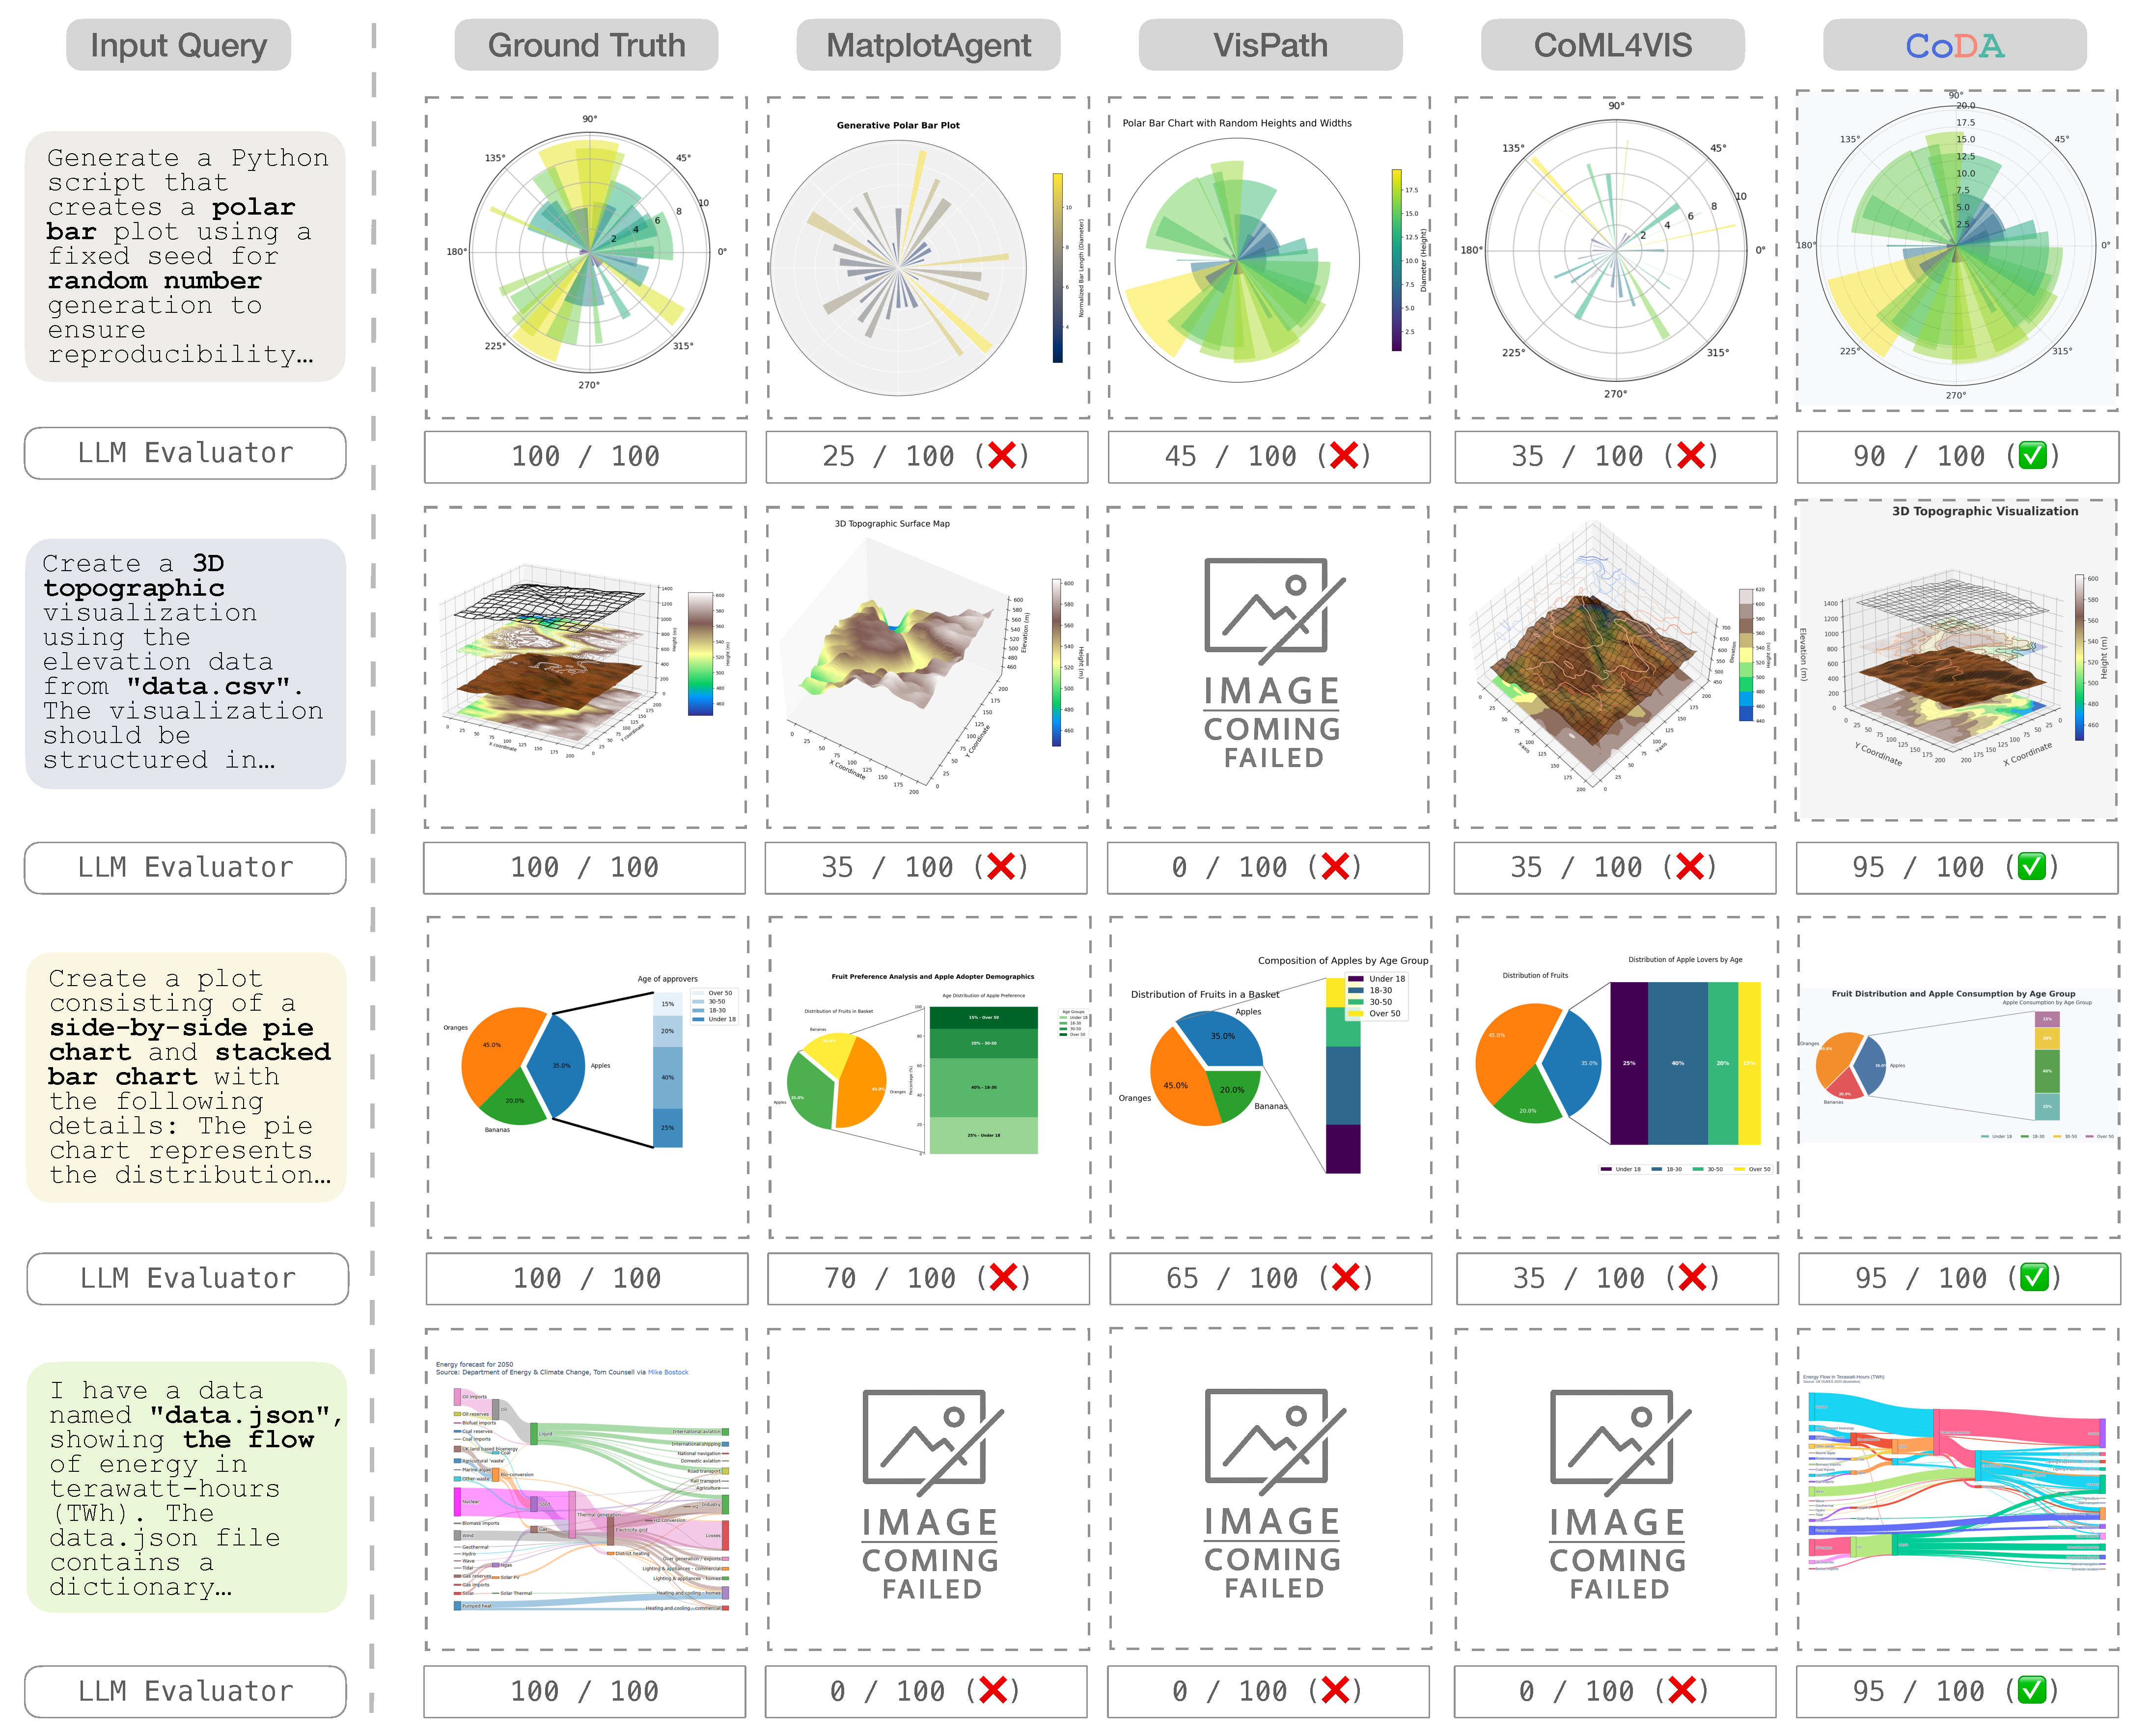
\includegraphics[width=1\linewidth]{figures/examples.pdf}
    \caption{Qualitative comparison of visualizations generated by baselines (\textit{MatplotAgent}, \textit{VisPath}, \textit{CoML4VIS}) and \methodname{}. Provided with a natural language query and data files (if has), models produce code to create plots. \methodname{} yields outputs that more faithfully capture complex patterns, chart types, and aesthetics, while baselines often fail on ambiguity, 3D structures, or multi-source integration. }
    \label{fig:placeholder}
    % \vspace{-10pt}
\end{figure}

Data visualization plays an important role in business intelligence, data science and decision-making, enabling professionals to uncover insights from complex datasets through intuitive graphical representations~\citep{ramesh2024challenges,gahar2024open,jambor2024zero,beschi2025characterizing,10747692}. 
In practice, data analysts might spend over two-thirds of their time on low-level data preparation and visualization tasks, often iterating manually to achieve clarity, accuracy, and aesthetic appeal~\citep{LaiLYC25,rezig2021technical,lee2021survey}. This ``unseen tax'' diverts focus from insight generation, highlighting the critical need for automated systems that can transform natural language queries and complex data into effective visualizations~\citep{wu2024automated,chen2024viseval,wang2023natural}.
With the rise of large language models (LLMs)~\citep{naveed2025comprehensive,achiam2023gpt,team2024gemma,comanici2025gemini}, there is immense potential to automate this pipeline. However, realizing this potential requires addressing core challenges: (1) handling large datasets, (2) coordinating diverse expertise (e.g., linguistics, statistics, design), and (3) incorporating iterative feedback to refine outputs against real-world complexities like messy multi-file data and complex visualization needs.



Current approaches to automate visualization suffer from various limitations. Traditional rule-based systems, such as Voyager~\citep{10.1145/3025453.3025768,7192728} and Draco~\citep{yang2023draco}, formalize design knowledge as constraints but remain confined to predefined templates, struggling with natural language queries or diverse data patterns~\citep{wu2024automated,hoque2025natural}. 
LLM-based methods, like CoML4VIS~\citep{chen2024viseval}, leverage chain-of-thought prompting to generate visualizations~\citep{comanici2025gemini}, but often ingest raw data directly, risking token limit violations, hallucinations, and multi-source data faltering~\citep{bai2024hallucination,chen2024viseval}.
Multi-agent frameworks, such as VisPath and MatplotAgent, introduce collaboration system to generate plot code but lack metadata-focused analysis, leading to overfitting in data processing and weak persistence against iterative edits~\citep{seo2025automated,yang2024matplotagent}. 
We argue these issues stem from a common limitation in current agentic visualization systems: they concentrate reasoning and coordination on initial query parsing, which proves insufficient for handling complex data environments (e.g., multiple and large files), code errors, and iterative refinement. This design limits their ability to
adapt to unexpected data challenges.


To address these challenges and limitations, we propose \methodname{} (\textbf{\textcolor{StarIndigo}{Collaborative} \textcolor{StarCoral}{Data-visualization} \textcolor{StarTeal}{Agents}}), a multi-agent system that deepens visualization by projecting tasks into a self-evolving pipeline where agents specialize in understanding, planning, generating, and reflecting. 
By analyzing metadata schemas and statistics without raw data file uploads, we circumvent context window limit of LLMs; specialized agents enhance domain reasoning; and image-based evaluation verifies the completion from a human perspective. This builds a robust framework for complex, iterative, and multi-source agentic visualizations, where agents collaborate deeply to ensure visualization quality.
The key contributions of this work are as follows:
\begin{itemize}[itemsep=0pt, parsep=0pt, topsep=0pt, leftmargin=2em]
    \item We propose \methodname{}, an extensible framework with specialized agents for metadata analysis, task planning, code generation and debugging, and self-reflection, enabling robust handling of complex data and visualization needs (See Figure~\ref{fig:placeholder} and Appendix~\ref{appendix:add} for qualitative analyses).
    \item Extensive experiments on MatplotBench and Qwen Code Interpreter benchmarks yield substantial gains in the Overall Score over strong baselines such as \textit{MatplotAgent}, \textit{VisPath}, and \textit{CoML4VIS}, with maximum improvements of 24.5\%, 41.5\%, and 26.5\% respectively. Furthermore, CoDA significantly outperforms competitive baselines on the DA-Code Benchmark, which features complex, real-world Software Engineering scenarios.
    \item A comprehensive ablation study validates the necessity of CoDA's core components. Results demonstrate that self-evolution, the global TODO list, and the example search agent each provide a statistically significant positive impact on overall performance.
\end{itemize}

